\documentclass[10pt]{article}
\usepackage{a4}
\usepackage{epsfig}
\usepackage{listings}
\lstset{language=Delphi}%
\lstset{basicstyle=\sffamily\small}%
\lstset{commentstyle=\itshape}%
\lstset{keywordstyle=\bfseries}%
\lstset{blankstring=true}%
\newif\ifpdf
\ifx\pdfoutput\undefined
  \pdffalse
\else
  \pdfoutput=1
  \pdftrue
\fi
\begin{document}
\title{Programming GTK in Free Pascal}
\author{Florian Kl\"ampfl\\and\\Micha\"el Van Canneyt}
\date{July 2000}
\maketitle
\section{Introduction}
The GTK library is a popular widget library for the X-Windows system.
It is used as the basis for the GIMP graphical manipulation program 
and for the GNOME application framework. With its ports to Microsoft 
Windows and BeOS, it allows to program a graphical interface for any
application in a platform independent way.

GTK is implemented in C, but it is possible to access its functionality from
Free Pascal. For this, its headers have been translated to Pascal,
so a program written in Free Pascal can make use of the functionality 
offered by GTK and its companion libraries GDK and GLIB. In fact, there is
an open source project (Lazarus) which makes use of GTK in order to build
an open-source alternative to the visual classes offered by Inprise's
Delphi.

This article intends to present an introduction to programming GTK in
Free Pascal. It by no means covers all of the functionality that GTK 
offers, as this would probably require a complete manual.

The first section gives some general considerations on the GTK toolkit.

\section{GTK is a C library}
Since GTK is an external library, some import units describing the calls in
the libraries are needed. Three libraries make up the GTK programming kit:
\begin{description}
\item[glib] this library contains some general programming tools, and
defines platform independent types, which are used throughout the other
libraries. To use this library, it is sufficient to include the 
\lstinline|glib| unit in your \lstinline|uses| clause.
\item[gdk] encapsulates the Windowing system (X or Windows) underlying GTK. 
It contains routines to draw on the screen, and react to various mouse or 
keyboard events. To use these
routines, the \lstinline|gdk| unit must be included in the \lstinline|uses|
 clause of a unit or program.
\item[gtk] contains the widget library. This is a series of controls such
as edit boxes, drop-down lists and many more, which are organised in an OOP
structure. Since the library is written in C, there is no programming 
language support for this structure.

All definitions of the gtk library are contained in the gtk unit, which
must be included in the \lstinline|uses| clause of any program or unit that needs their
functionality.
\end{description}

The GTK toolkit was programmed in C. This has some consequences for the
Pascal interface, since some C constructs do not port easily to Pascal.
When using the Pascal translation of the C headers, the following must be
kept in mind:

\begin{enumerate}
\item Reserved words: Pascal reserved words in types, record element names
etc. have been prepended with the word 'the'. For example \lstinline|label|
becomes \lstinline|thelabel|.
\item Functions and procedures have been kept with the same names. 
\item Types have been prepended with T, that is, the C type
\lstinline|GtkWidget| has become \lstinline|TGtkWidget|.
\item Pointers to types have been defined as the type name, prepended with a
P.  \lstinline|GtkWidget *| becomes \lstinline|PGtkWidget|. 
\item Records with bit-size elements: C allows to store parts of a record in 
individual bits; whereas in Pascal, the minimum size of an element in a
record is a byte. To accommodate this, functions were defined to retrieve
or set single bits from a record. The functions to retrieve a bit
have the name of the record field. The procedure to set a bit has 
the name of the field prepended with 'set\_'.
For example
\begin{lstlisting}[language=c]{cpackedstruct}
struct SomeStruct
{
  gchar *title;
  guint visible        : 1;
  guint resizeable     : 1;
};
\end{lstlisting}
translates to 
\begin{lstlisting}{ppackedstruct}
TSomeStruct = record
 title : Pgchar;
 flag0 : word;
end;
function  visible(var a: TGtkCListColumn): guint;
procedure set_visible(var a: TGtkCListColumn; __visible: guint);
function  resizeable(var a: TGtkCListColumn): guint;
procedure set_resizeable(var a: TGtkCListColumn;__resizeable: guint);
\end{lstlisting}
\item Macros. Many C macros have not been translated. The typecasting 
macros have been dropped, since they're useless under Pascal. 
Macros to access  record members have been translated, but they are to be
considered as {read-only}. So they can be used to retrieve a value, but 
not to store one. e.g. 
\begin{lstlisting}{macro}
function GTK_WIDGET_FLAGS(wid : pgtkwidget) : longint;
\end{lstlisting}
can be used to retrieve the widget flags, but not to set them. so things like 
\begin{lstlisting}{invaliduseofmacro}
GTK_WIDGET_FLAGS(wid):=GTK_WIDGET_FLAGS(wid) and someflag;
\end{lstlisting}
will not work, since this is a function, and NOT a macro as in C. 
\item Calling conventions: A C compiler uses another calling convention 
than the Free Pascal compiler. Since many GTK functions need a callback,
these callback must use the C calling convention. This means that every
function that is called by GTK code, should have the \lstinline|cdecl| 
modifier as a part of its declaration.
\end{enumerate}

Compiling a GTK application is no different than compiling any other Free
Pascal application. The only thing that needs to be done is to tell the free
Pascal compiler where the gtk, gdk and glib libraries are located on your
system. This can be done with the \verb|-Fl| command-line switch. For
example, supposing the gtk library is located in \verb|/usr/X11/lib|, the
following command-line could be used to compile your application:
\begin{verbatim}
ppc386 -Fl/usr/X11/lib mygtkapp.pp
\end{verbatim}
This example supposes that the gtk unit is be in your unit search path. If
it is not, you can add it with the \verb|-Fu| switch.

\section{The bricks of a GTK application}
The building-blocks of a a GTK application are the {\em widgets}. 
Widgets are the equivalent of Delphi's controls. And although GTK 
is not an object oriented library, the library defines a record 
\lstinline|TGtkWidget| which contains all settings common to all
widgets; all widgets start with this record, and add their own 
specific data to it. This creates a tree-like structure with all 
the widgets present in the GTK library, to which your own widgets 
can be added.

All functions that create a particular widget return a pointer
to a \lstinline|TGtkWidget| record. It is not recommended to 
manipulate the contents of the widget record directly; GTK offers 
many functions to manipulate the members of the record, e.g.  
\lstinline|gtk_widget_set_parent| or \lstinline|gtk_widget_get_name|.
To this set of functions, each new widget adds a few functions that are 
specific to this particular widget. 

Each widget has a specific function and a specific look; there are many
widgets to choose from. A complete list of widgets is outside the scope of
this article; the GTK reference manual offers an overview of available
widgets. In general it can be said that most widgets one would expect
are present in the GTK library: Edit fields, buttons, check-boxes, various 
lists, menus, combo-boxes, tree views, and some pre-defined dialogs. 

Any of these widgets is created with a \lstinline|gtk_WIDGET NAME_new| call. 
This call can accept arguments; The number and type of arguments depend 
on the widget. 
For example, to create a button that displays a text, the call is defined 
as follows:
\begin{lstlisting}{}
gtk_button_new_with_label(ALAbel : PChar)
\end{lstlisting}
All widgets can be destroyed with the \lstinline|gtk_widget_destroy| call,
irrespective of their type.

\section{Showing things on the screen}
To show things on the screen, it is necessary to create a window. A window
is created with the the \lstinline|gtk_window_new| call. This call accepts 
as an argument the type of window to be created. 

Creating a window creates it's structure in memory, but doesn't show it on 
screen. To show this window on the screen,a call to the 
\lstinline|gtk_widget_show| function is needed, as can been seen in
example 1.
\lstinputlisting{gtkex/ex1.pp}
If the window contains widgets, the \lstinline|gtk_widget_show| function
must be called for each widget. 

Looking at example 1, one notices 2 special calls: \lstinline|gtk_init| and
\lstinline|gtk_main|. These calls should be present in any program that uses
the GTK library.  

The first call initialises the GTK library. Among other things, it reads
the command-line to see e.g. which display should be used.

The second call is the heart of the GTK widget library: It starts the
message loop of GTK. This call will not return, unless somewhere else
in the program \lstinline|gtk_main_quit| is called. As long as the call
doesn't return, GTK will wait for events such as mouse clicks, key-presses
and so on. It will handle these events, but it will not notify you of any 
of these events except if you specifically ask for it. 

A window by itself is of course not very interesting. To make it more
interesting, some elements should be added. 

Adding a widget to a parent is done with the \lstinline|gtk_container_add|
call. This call places a widget in a container. A container is a widget 
which can contain other widgets; not all widgets are containers, however.

Example 2 shows how to add a widget (a button) to a container (the window
in this case). It also shows that the container has some specific
properties, which can be manipulated as well (in this case, the border
width). Since not each widget is a container, the window pointer must be
typecasted to \lstinline|GTK_CONTAINER| in order to be accepted by the
container handling calls.

\lstinputlisting{gtkex/ex2.pp}

Adding more than 1 widget to a container is not trivial in GTK. The reason
for this is that GTK has not been designed to set widgets at a specific
location in their parent widget. Instead, GTK asks that you 'pack' your
objects in their parent widget. This means that if the parent widget is
resized, it's child widgets are resized as well, depending on the packing
options that were set.

One of the reasons that the GTK library was set up this way, is that the
size of a widget is not well-defined. For instance, the size of a button
depends on whether it is the default widget of the window or not. Given 
that this is so, the placement of such a button is not well-defined either.

The most common ways of packing widgets in a parent widget are the
following:
\begin{enumerate}
\item using a vertical box.
\item using a horizontal box.
\item using a table.
\end{enumerate}
We'll discuss these ways in the subsequent. There are other ways, but these
are probably the most important ones.

\subsection{Using boxes}

A horizontal or vertical box can be used to contain a row or column of
widgets. Various options can be set to modify the spacing between the 
widgets, the alignment of the widgets in the box, or the behaviour of 
the box when the user resizes the parent widget. Boxes work only in 
one direction. The widgets inside a horizontal box always have the height of
the box, and widgets in a vertical box always have the width of the vertical
box.

You can create a horizontal box with the \lstinline|gtk_hbox_new| call. 
It accepts 2 arguments: The first one is a boolean. It tells GTK whether the
children should have the same space in the box. The second one is an
integer, which tells GTK how much space to leave between the widgets in the
box. Likewise, a vertical box can be created with the
\lstinline|gtk_vbox_new| call. This call accepts the same arguments as the
first box.

Adding widgets to a box happens with the \lstinline|gtk_box_pack_start| or
\lstinline|gtk_box_pack_end| calls. The former adds a widget at the start
of the box, the latter adds a widget at the end of the box. Both functions
accept the same arguments:
\begin{lstlisting}{boxarguments}
(Box : PGtkBox; Widget: PGtkWidget;
 expand gboolean; fill : gboolean;padding : guint);
\end{lstlisting}
The \lstinline|expand| argument tells the box whether it should take the
size of it's parent widget, or whether it should resize itself so that it is
just large enough to fit the widgets. The latter allows to justify the
widgets in the box (but only if the box is {\em not} homogeneous.  
If the box should keep the size of it's parent, then the \lstinline|fill| 
argument decides what is done with the extra space available. 

If \lstinline|fill| is \lstinline|True| then the extra space is
divided over the widgets. If \lstinline|fill| is \lstinline|False| then the
extra space is put in between the widgets. 

The \lstinline|padding| adding tells the box to add extra space for this 
particular widget.

The following program shows the use of a box:
\lstinputlisting{gtkex/ex3.pp}
What the program does is the following: It creates a window, which it splits
up in two halves by means of the \lstinline|totalbox| widget. This is a
vertical box, which will contain two other boxes: a vertical box and a
horizontal box. Each of these two boxes is filled with buttons.
The behaviour of the boxes can be seen when the window is resized.

The effect of the various arguments to the pack calls can be seen by
changing the arguments and recompiling the example.

\subsection{Using tables}
A table is used to set widgets in a grid inside the parent widget. It acts
like a grid with cells, in which you can 'hang' your widgets. If the user 
resizes the parent widget, then the size of the grid cells changes, and 
the widgets will change their location and size, based on the size of the 
new grid cells. 

To create a table to manage a window's layout, the \lstinline|gtk_table_new|
call is used. It accepts 3 arguments: the number of rows, the number of
columns and a boolean which tells GTK whether the cells should always have
the same size or not. 

To add a widget to a table, the \lstinline|gtk_table_attach| call is used.
It is declared as
\begin{lstlisting}{}
gtk_table_attach(Table: PGtkTable;Widget: PGtkWidget;
                 Left, right, top, bottom : guint;
                 Xoptions,Yoptions : TGtkAttachOptions;
                 Xpadding,Ypadding : Guint);
\end{lstlisting}
The first two options of this call are self-explanatory. The next four
options, however, need some explanation. Contrary to what the name 'table'
suggests, these do {\em not} specify the coordinates of cells; instead, they
specify the grid lines that delimit the cells. 

\begin{figure}
\caption{Placing widgets in a table.\label{fig:table}}
\begin{center}
\ifpdf
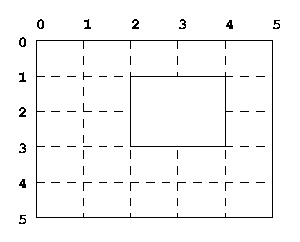
\epsfig{file=table.pdf}
\else
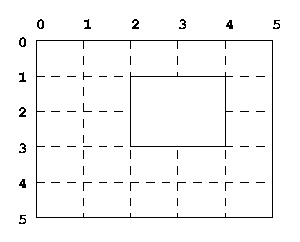
\epsfig{file=table.eps}
\fi
\end{center}
\end{figure}

Figure \ref{fig:table} represents a table with 5 rows and 5 columns, with
cells of the same size. The call to create this table could be:
\begin{lstlisting}{}
maintable:=gtk_table_new(5,5,TRUE);
\end{lstlisting}
To hang a widget in this table, so it starts in cell (2,1) and ends in cell
(3,2), where the cells are counted starting with 0, it is necessary to tell 
GTK that the widget starts at horizontal grid line 2, and ends at horizontal
grid line 4. Vertically, it starts at grid line 1, and ends at grid line 3. 
This means that the following call would place the widget at its correct
location:
\begin{lstlisting}{}
gtk_table_attach(maintable,mybutton,
                 2,4,1,3,
                 GTK_EXPAND OR GTK_FILL,GTK_EXPAND OR GTK_FILL,
                 0,0);
\end{lstlisting}
GTK delivers a shorter form of this call:
\begin{lstlisting}{}
gtk_table_attach_defaults(maintable,mybutton,2,4,1,3);
\end{lstlisting}
The parameter \lstinline|GTK_EXPAND or GTK_FILL| tells GTK that the widget 
should always take up the full space assigned to it.

The following example program illustrates the use of a table in a gtk
application:
\lstinputlisting{gtkex/ex4.pp}
The example creates a table with 6 rows and 6 columns. It places 3 buttons, 
each at a different location in the table, with different sizes. The first
button has a width and height of 1 cell and is located at cell (1,1). The 
second has a width and height of two cells, and is located at cell (3,1).
The last button is 4 cells wide and has a height of 1 cell, and is located
at cell (1,4). When the window is resized, the cells are resized as well,
and the buttons follow the size of the cells.

{\em Remark:} because the table has homogeneous cells, the minimum width 
and height of the cells is determined by the first button (in this case). 
Since all cells must have the same size, this means that the minimum size 
of the window is 6 times the size of the first button (plus a border).

\section{Reacting to user input}
So far, the example programs did not react to button clicks or any other user
action other than closing the window. To make a window respond to user
actions, it is necessary to install signal callbacks or event handlers.

The difference between signals and events is that signals come from the GTK
toolkit. Events come from the underlying window system (X or Windows).
For example, 'button\_pressed' is an event that is generated by the window
system when the user clicks with his mouse. It is possible to react to 
this event. 

On the other hand, a button widget defines a signal 'clicked'. 
The 'clicked' event will occur when the user clicks on the button. 
So, many signals that are defined by GTK widgets are just a translation 
of events to something specific for that widget.

Since calls to connect to a signal or to an event are the same, in what
follows the discussion will be restricted to signals, but all that is 
said is also true for events.

GTK has essentially 2 ways to install signal callbacks. The only difference
between these calls is the arguments that the callback function accepts.

The first way to install a callback is using the
\lstinline|gtk_signal_connect| function. This function is declared as
follows:
\begin{lstlisting}{}
TGtkSignalFunc = procedure ;cdecl;
Function gtk_signal_connect(TheObject:PGtkObject;Name:Pgchar;
                            Func:TGtkSignalFunc;Data:gpointer):guint;cdecl;
\end{lstlisting}

The first argument of this call (\lstinline|TheObject|) is the object 
(usually a widget) to which you want to assign an event handler. The second
parameter, \lstinline|Name|, is the event you wish to catch with this
callback (an example could be 'clicked' for a button). The third argument
(\lstinline|Func|) is the function that should be called when the event occurs. 
The \lstinline|Data| argument is a pointer to arbitrary data. This pointer
will be passed on to the callback function \lstinline|func| when the event
occurs.

The \lstinline|gtk_signal_connect| function returns an integer. This integer 
is the number of the callback for this event. It is possible to attach more 
than one callback to an event in GTK. When the event occurs, the callbacks 
will be executed in the order that they have been attached to the widget. 

The declaration of the \lstinline|TGtkSignalFunc| type requires that every
callback function that is passed to GTK must be typecast. Since GTK defines
only one function to set a signal handler, this is necessary, since
callbacks can have different forms. This mechanism is error-prone, since
in this manner it is possible to pass a function to GTK which has the wrong
number of arguments.

However, most callbacks must be of the form:
\begin{lstlisting}{}
Function (Widget : PGtkWidget; Data : GPointer) : guint;cdecl;
\end{lstlisting}
Such a callback function accepts 2 arguments: the first argument
(\lstinline|Widget|) is the widget which caused the event 
(for example, the button which was clicked). The second argument is a
pointer to arbitrary data. This is the pointer that was passed as
\lstinline|Data| when the callback was installed.

Signals are identified by their name. The GTK reference guide contains a
complete list of supported signals.

The first example shows how a handler for the 'destroy' signal of the
window is installed. When the window-manager kills the window, this 
signal is sent. The \lstinline|gtk_main_quit| instructs GTK that it 
should stop processing X events and exit the \lstinline|gtk_main| call.

A second method to connect a callback to a signal is using the
\lstinline|gtk_signal_connect_object| call. This call is defined as
follows:
\begin{lstlisting}{}
Function gtk_signal_connect_object(theobject:PGtkObject;
                                   name:Pgchar;
                                   func:TGtkSignalFunc;
                                   slot_object:PGtkObject):guint;cdecl
\end{lstlisting}
It is similar in function to the \lstinline|gtk_signal_connect| function,
only it doesn't allow to pass arbitrary data to the signal handler. Instead,
the handler must {\em always} be of the following form:

\begin{lstlisting}{}
Function (AnObject : PGtkObject);
\end{lstlisting}
The \lstinline|slot_object| pointer that was provided in the call to
\lstinline|gtk_signal_connect_object| will be passed as the
\lstinline|AnObject| argument to this function. Many GTK functions have the
above form; this makes it possible to attach a GTK internal function to a
signal.

To illustrate this, the second example is modified so that clicking the button
will also close the window:
\lstinputlisting{gtkex/ex5.pp}
In the example, the call to \lstinline|gtk_signal_connect_object| will
connect the 'clicked' signal of the button to the
\lstinline|gtk_widget_destroy| function of GTK, and passes the pointer to
the window widget to it. When the user clicks the button, the
\lstinline|gtk_widget_destroy| function will be called with as argument the
pointer of the window object. As a result, the window widget will be
destroyed, it's 'destroy' signal will be activated, and the
\lstinline|gtk_main_quit| function will be called through the program's
'destroy' handler for the window.

Since the signal handler connect call returns an integer by which it can 
be identified, it is possible to manipulate or even remove the handler 
once it has been installed.

For instance it is possible to temporarily disable a signal handler with the 
\lstinline|gtk_signal_handler_block| call, and to enable it again with the
\lstinline|gtk_signal_handler_unblock| call. An example of how to do this
can be found in the following example:
\lstinputlisting{gtkex/ex6.pp}
There are other things that one can do with signal handlers, but a complete
discussion of all possibilities is outside the scope of this article.

Some widgets do not have their own window; i.e. they do not receive events
from the underlying windowing system. An example of such a widget is a
label. A label just draws it's text on it's parent widget, and nothing else.

To be able to respond to certain events, an event-box must be used, and the 
window-less widget must be placed in it. An event-box can be created with
the \lstinline|gtk_event_box_new| call. This call accepts no arguments.

To this event-box, a window-less widget can be added. The event-bow will
then capture events for the window-less widget. The following example shows
how to use an event-box to detect when the mouse pointer is moved over a
label:
\lstinputlisting{gtkex/ex7.pp}
If the mouse pointer is moved over the first label, the text of the second
label is adapted accordingly. The example also shows the use of
\lstinline|gtk_widget_show_all|, which shows a widget and all widgets
contained in it.

\section{A touch of style}
The look of a GTK application is controlled through the use of styles. A
style controls the colors in which a widget is drawn, in various states.
As an example: a widget may be drawn differently depending on whether it 
has focus or not. How to draw the widget in each of this states is described
in the style of the widget.

GTK recognizes the following states of a widget:
\begin{description}
\item[NORMAL] The normal state of a widget. No mouse over it.
\item[PRELIGHT] Is the state of a widget when the mouse is over it.
\item[ACTIVE] Is the state of a widget when it is pressed or
clicked.
\item[INSENSITIVE] if the widgets is disabled ('grayed').
\item[SELECTED] When the object is selected.
The GTK unit has a constant for each of these states; it is the above name
with \lstinline|GTK_STATE_| prefixed, so e.g. \lstinline|GTK_STATE_NORMAL|
for the normal state.

\end{description}


Each widget class has a default style in which it is drawn. If you wish to
change the way all these widgets look, you should change the default style
of this class. If you want to change the way one particular widget looks,
you should make a new style, and apply it to that particular widget. It is
possible to make a copy of an existing style and modify the copy before
applying it.

It is also possible to change the default style of widgets. Changing the
default style of widgets will have effect on all widgets created after the
new style was set. Widgets created before that will be unaffected.

The following example shows how to set the color of a label. It takes a
copy of the standard label style, and modifies it so the foreground color
becomes red. It then applies the modified style to the first label.
The second label is unaffected by this change
\lstinputlisting{gtkex/ex8.pp}

The last example shows how to change the color of a button when the mouse
moves over it.
\lstinputlisting{gtkex/ex9.pp}

\section{Carrying on}
In the previous sections, some basic concepts of GTK have been introduced.
However, GTK is a big toolkit and much more can be said about it. It is
outside of the scope of the current article to describe all Widgets in the
GTK library. The range of offered widgets is broad, and there probably is a
widget for each conceivable task. If there is a missing widget, it is always
possible to write a new widget. 

In principle, therefore, GTK is suitable to write large applications, also
when writing in Free Pascal. However, the fact that it is written in C and 
it's interface is C oriented, justifies the writing of a small Pascal Object 
Oriented wrapper around it. 
The following arguments show the need for such a wrapper:
\begin{enumerate}
\item C has no object-oriented language constructs. This makes it necessary
to do a lot of typecasts in GTK calls. Using Classes or Objects, this is no
longer necessary, and will improve code readability substantially.
\item C uses null-terminated strings. It can be useful to wrap calls that
need a null-terminated string into one that accepts a normal string as an
argument. Using ansistrings will make the conversion to null-terminated
strings easier.
\item The signal mechanism of GTK destroys the strong type checking of
Pascal. When compiling the statement 
\begin{lstlisting}{}
  Button.OnClick:=@MyForm.OnButtonClick
\end{lstlisting}
The compiler checks that the \lstinline|OnButtonClick| method can be
assigned to the \lstinline|OnClick| event. Under GTK, it is possible
to pass any function as a handler for a signal, as in
\begin{lstlisting}{}
gtk_signal_connect (PGTKOBJECT (window), 'destroy',
                    GTK_SIGNAL_FUNC (@destroy), NULL);
\end{lstlisting}
This can lead to errors if the \lstinline|destroy| procedure accepts a
different number of arguments, or other arguments than the ones that 
GTK provides. Therefore it would be a good idea to implement methods that
would force type checking, e.g:
\begin{lstlisting}{}
Button.AddOnClick(@MyForm.OnButtonClick);
\end{lstlisting}
Such a statement would only compile if the \lstinline|OnButtonClick| would
be of the right type.
\end{enumerate}
Additional benefits of making such a wrapper would be simpler code, and
hence better readability. Both improve the maintainability of the code as well,
which are all important factors when writing a large application.
\end{document}
